\documentclass[10pt,a4paper]{article}
\usepackage[utf8]{inputenc}
\usepackage[magyar]{babel}
\usepackage[T1]{fontenc}
\usepackage{amsmath}
\usepackage{amsfonts}
\usepackage{amssymb}
\usepackage{graphicx}
\begin{document}
\title{Méréstechnika laboratórium II 13. jegyzőkönyv}
\author{Koncz István Márton\\\\A2754O}
\date{\today}
\maketitle
\newpage
\section{13. sz. laboratóriumi mérés}
	Mérés dátuma:\date{2017.09.11}
	\subsection{A mérés célja}
	A digitális oszcilloszkóp kezelésének többlet funkcióinak
elsajátítása, a kapott mérési eredmények kiértékeléséhez
szükséges szemlélet kialakítása.
	\subsection{Mérési feladatok}
		\subsubsection{Az oszcilloszkóp csatorna-menük vizsgálata}
		\begin{enumerate}
			\item Beállítások változtatásának eredményei CH1 csatornán:
				$$$$ $$$$ $$$$ $$$$ $$$$
			\item Az 1V/DIV és a 10mV/DIV finom-beállítások közötti eltérések:\\\\
			\begin{tabular}{|c|c|}
			\hline 
			1V/DIV & 10mV/DIV \\ 
			\hline 
			 &  \\ 
			\hline 
			 &  \\ 
			\hline 
			 &  \\ 
			\hline 
			\end{tabular}
			\item A függőleges pozíció állításához tartozó megfigyeléseim:
				$$$$ $$$$ $$$$		 
		\end{enumerate}
		\subsubsection{Horizontális menü vizsgálata}\newpage
		\begin{enumerate}
			\item A Window megjelenítés hatása, rajzzal:
			\\\\
						\begin{figure}[hbtp]
						\centering
				    		 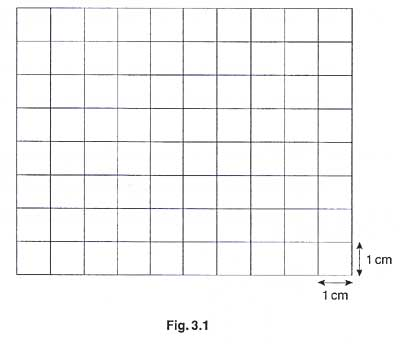
\includegraphics[scale=0.5]{teljes/osc.jpg}
						\caption{Ablaktartomány beállításakor}
						\end{figure}
			\\
					\begin{figure}[hbtp]
					\centering
					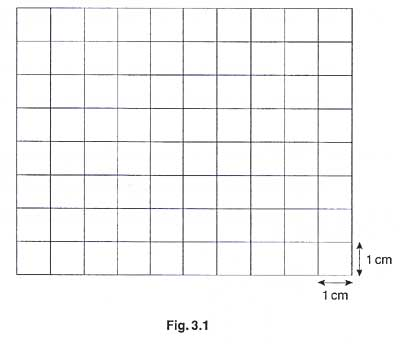
\includegraphics[scale=0.5]{teljes/osc.jpg}
					\caption{Ablak megjelenítésekor}
					\end{figure}\\\\
			\item Sec/DIV hatása: $$$$ $$$$
			\item Autoset hatása, rajzzal:
			Autoset hatására az ábra értékelhetetlen. A megállításhoz szükséges holdoff idő: $6,950 \mu s$ \\\\\begin{figure}[hbtp]
			\centering
			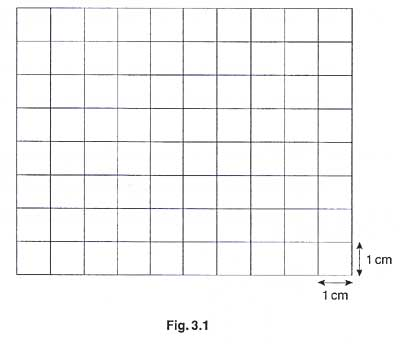
\includegraphics[scale=0.5]{teljes/osc.jpg}
			\caption{Autoset}
			\end{figure}
					
		\end{enumerate}
		\subsubsection{Az utótriggerelés, az előtriggerelés és a késleltetett utótriggerelés vizsgálata}
			\begin{enumerate}
				\item A vízszintes pozíció állító működésének vizsgálata:\\
				$$$$ $$$$ $$$$ $$$$
				\item Set to Zero vizsgálata: $$$$ $$$$ $$$$ $$$$
				\newpage
				\item Az oszcilloszkóp jelalakjainak vizsgálata:
				\\\\
				\begin{figure}[hbtp]
				\centering
				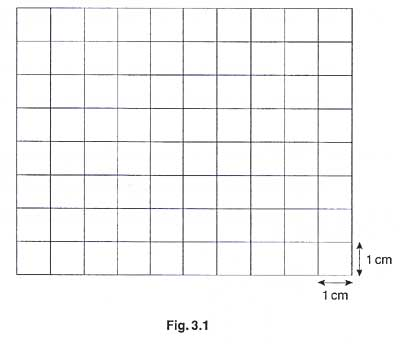
\includegraphics[scale=0.5]{teljes/osc.jpg}
				\caption{1MHz négyszögjel}
				\end{figure}
				\begin{figure}[hbtp]
				\centering
				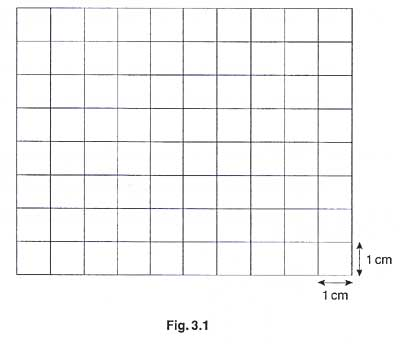
\includegraphics[scale=0.5]{teljes/osc.jpg}
				\caption{QA}
				\end{figure}
				\newpage
				\begin{figure}[hbtp]
				\centering
				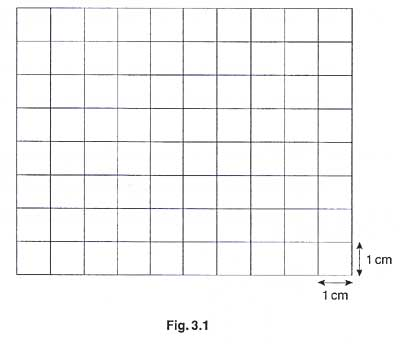
\includegraphics[scale=0.5]{teljes/osc.jpg}
				\caption{QB}
				\end{figure}
				\begin{figure}[hbtp]
				\centering
				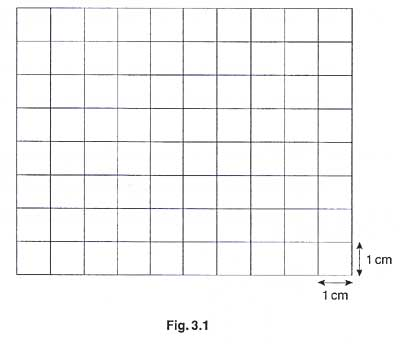
\includegraphics[scale=0.5]{teljes/osc.jpg}
				\caption{QC}
				\end{figure}
				\newpage
				\begin{figure}[hbtp]
				\centering
				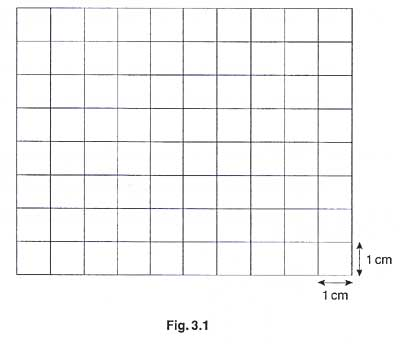
\includegraphics[scale=0.5]{teljes/osc.jpg}
				\caption{QD}
				\end{figure}
				\item A jel a képernyőn kívüli részeinek vizsgálata: $$$$ $$$$ $$$$
			\end{enumerate}
			\subsubsection{A trigger menü vizsgálata}
			\begin{enumerate}
				\item Nagy és kisfrekvenciás elnyomás határfrekvenciájának mérése.\\\\\begin{tabular}{|c|c|}
				\hline 
				Triggerforrás & CH1 \\ 
				\hline 
				Trigger él & emelkedő \\ 
				\hline 
				Triggerelési üzemmód & Auto \\ 
				\hline 
				Triggerjel csatolása & $$$$ \\ 
				\hline 
				\end{tabular}  
				\item 1 kHz-es négyszögjel vizsgálata CH1 csatornán$$$$
			\end{enumerate}
			\subsubsection{Kibővített matematikai funkciók vizsgálata}
			A Math Menu gomb 3 funkciót kínál: összegzés, különbségképzés, FFT spektrum analízis.
			\subsubsection{Automatikus gyorsmérések elvégzése}
			\begin{tabular}{|c|c|c|}
			\hline 
			Mennyiség & Szinuszjel & Négyszögjel \\ 
			\hline 
			f & $1 kHz$ & $10 kHz$ \\ 
			\hline 
			T & $1 ms$ & $100 \mu s$ \\ 
			\hline 
			Mean & &  \\ 
			\hline 
			Pk-Pk &  &  \\ 
			\hline 
			Cyc RMS &  &  \\ 
			\hline 
			Min &  &  \\ 
			\hline 
			Max &  &  \\ 
			\hline 
			Rise time &  &  \\ 
			\hline 
			Fall time &  &  \\ 
			\hline 
			Pos Width &  &  \\ 
			\hline 
			Neg Width &  &  \\ 
			\hline 
			\end{tabular} 
			$$$$
			Négyszögjel felfutási idejének mérése:\\\\
			\begin{tabular}{|c|c|}
			\hline 
			TIME/DIV & Négyszögjel felfutási ideje \\ 
			\hline 
			$50 \mu s$ &  \\ 
			\hline 
			$25 \mu s$ &  \\ 
			\hline 
			$10 \mu s$ &  \\ 
			\hline 
			$5\mu s$ &  \\ 
			\hline 
			\end{tabular}
			
			$$$$
			Magyarázat:
			\newpage
			$$$$
			A mérés értékelése:

\end{document}